\documentclass[UTF8,fontset=none,12pt]{ctexart}

\setCJKmainfont{Songti SC}
\setCJKsansfont{PingFang SC}
\setCJKmonofont{Songti SC}

\usepackage[a4paper,margin=2.35cm]{geometry}
\usepackage{amsmath,amssymb,amsthm,mathtools,bm}
\usepackage{graphicx}
\usepackage{float}
\usepackage{booktabs}
\usepackage{array}
\usepackage{enumitem}
\usepackage[hidelinks]{hyperref}

\newcommand{\epsmach}{\varepsilon_{\mathrm{machine}}}

\title{数值线性代数\quad 第 27 讲：Rayleigh 商与逆迭代}
\author{Lloyd N. Trefethen、David Bau III\quad 中文阅读版}
\date{}

\begin{document}
\maketitle
\pagestyle{plain}

本讲介绍几个经典的特征值算法。它们各自在特定场景下很有用，尤其是
逆迭代：当某个特征值已经知道时，逆迭代是计算对应特征向量的标准方法。
把这些工具组合起来，就得到著名的 QR 算法；QR 算法将在接下来的两讲中
讨论。

\section*{限制到实对称矩阵}

在数值线性代数中，大多数算法思想既适用于一般矩阵，也适用于经过一些
简化的 Hermitian 矩阵。对于本讲以及接下来的三讲，这种情形仍然成立，
但一般矩阵与 Hermitian 矩阵之间的差异会比较明显。因此，本四讲暂时只
考虑实对称矩阵，并且始终假设所用范数为 2-范数：

\[
A=A^T\in\mathbb{R}^{m\times m},\qquad
x\in\mathbb{R}^m,\qquad x^*=x^T,\qquad
\|x\|=\sqrt{x^Tx}.
\]

特别地，$A$ 的特征值都是实数，并且存在一组完备的正交特征向量。记

\[
\text{实特征值：}\ \lambda_1,\ldots,\lambda_m,
\qquad
\text{标准正交特征向量：}\ q_1,\ldots,q_m.
\]

特征向量按 $\|q_j\|=1$ 归一化；特征值的排序将在需要时具体说明。

接下来几讲的大多数思想属于第 25 讲介绍的两个阶段中的第二阶段。也就是
说，真正应用这些思想时，$A$ 不仅是实对称矩阵，通常还已经是三对角矩阵。
三对角结构有时具有数学上的重要性，例如可以帮助选择 QR 算法的移位；
它始终具有算法上的重要性，因为它可以把许多步骤的工作量从 $O(m^3)$
降到 $O(m)$，本讲末尾会具体说明。

\section*{Rayleigh 商}

向量 $x\in\mathbb{R}^m$ 的 Rayleigh 商定义为标量

\begin{equation}
 r(x)=\frac{x^TAx}{x^Tx}.
\tag{27.1}
\end{equation}

如果 $x$ 是特征向量，那么 $r(x)=\lambda$，其中 $\lambda$ 是对应的特征值。
这个公式的一种动机是：给定 $x$，什么标量 $\alpha$ 最像 $x$ 对应的“特征值”，
使得 $\|Ax-\alpha x\|_2$ 最小？这是一个形如
$x\alpha\approx Ax$ 的 $m\times1$ 最小二乘问题，其中 $\alpha$ 是未知标量，
而 $Ax$ 是右端项。对这个系统写出正规方程（式 (11.9)），就得到
$\alpha=r(x)$。因此，如果 $x$ 接近但不一定等于特征向量，$r(x)$ 是一个
自然的特征值估计。

为了定量研究这个想法，把 $x\in\mathbb{R}^m$ 看作变量，于是 $r$ 是从
$\mathbb{R}^m$ 到 $\mathbb{R}$ 的函数。我们关心 $x$ 接近特征向量时
$r(x)$ 的局部行为。对坐标 $x_j$ 求偏导：

\[
\frac{\partial r(x)}{\partial x_j}
=\frac{2(Ax)_j}{x^Tx}-\frac{2(x^TAx)x_j}{(x^Tx)^2}
=\frac{2}{x^Tx}\bigl(Ax-r(x)x\bigr)_j.
\]

把这些偏导数组成一个 $m$-向量，就得到 $r(x)$ 的梯度：

\begin{equation}
 \nabla r(x)=\frac{2}{x^Tx}\bigl(Ax-r(x)x\bigr).
\tag{27.2}
\end{equation}

由此可见，在 $A$ 的特征向量处，$r(x)$ 的梯度为零。反过来，如果
$x\ne0$ 且 $\nabla r(x)=0$，那么 $x$ 就是特征向量，$r(x)$ 是对应的特征值。

从几何上看，$A$ 的特征向量是函数 $r(x)$ 的驻点，而特征值是 $r(x)$
在这些驻点处的函数值。由于 $r(x)$ 与 $x$ 的尺度无关，驻点实际上位于
经过原点的直线上。若把 $x$ 限制在单位球面 $\|x\|=1$ 上，那么在特征值
互异时，这些驻点就成为彼此孤立的点：

\begin{figure}[H]
    \centering
    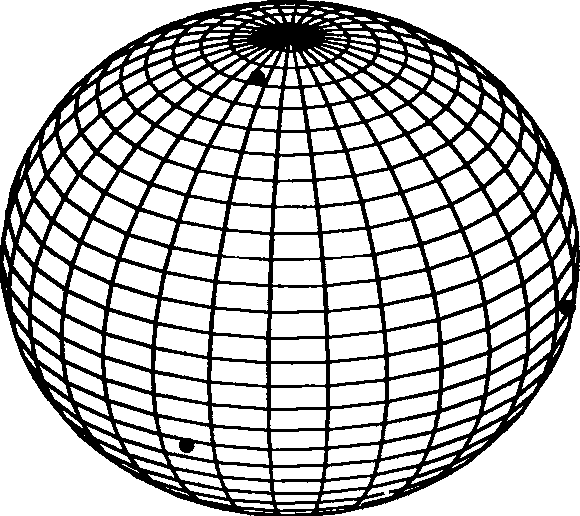
\includegraphics[width=0.47\linewidth]{../assets/figure-27-rayleigh-sphere.png}
    \caption{单位球面上的 Rayleigh 商。$r(x)$ 在 $\|x\|=1$ 上连续，
    其驻点是归一化特征向量；图示 $m=3$ 时的三个正交驻点及其对跖点。}
\end{figure}

令 $q_j$ 是 $A$ 的一个特征向量。由 $\nabla r(q_j)=0$ 以及 $r(x)$ 的光滑性
（除了原点 $x=0$ 外处处光滑），可得一个重要结论：

\begin{equation}
 r(x)-r(q_j)=O\bigl(\|x-q_j\|^2\bigr),\qquad x\to q_j.
\tag{27.3}
\end{equation}

因此，Rayleigh 商是特征值的二阶精度估计；这正是它强大的地方。

还可以更直接地推导 (27.3)。把 $x$ 展开为 $A$ 的特征向量
$q_1,\ldots,q_m$ 的线性组合。若
$x=\sum_{j=1}^m a_jq_j$，则

\[
r(x)=\frac{\sum_{j=1}^m a_j^2\lambda_j}{\sum_{j=1}^m a_j^2}.
\]

所以 $r(x)$ 是 $A$ 的特征值的加权平均，权重是 $x$ 在特征向量基下坐标
的平方。正因为坐标被平方，如果对所有 $j\ne J$ 都有
$|a_j/a_J|\le\epsilon$，那么
$r(x)-r(q_J)=O(\epsilon^2)$。

\section*{幂迭代}

现在换一个方向。设 $v^{(0)}$ 是满足 $\|v^{(0)}\|=1$ 的向量。下面的过程
称为幂迭代；第 25 讲开头曾把它作为一个不太好的想法提到过。幂迭代
有望产生一个序列 $v^{(k)}$，使其收敛到对应于 $A$ 的最大特征值的特征向量。

\paragraph{算法 27.1（幂迭代）}
\begin{verbatim}
v^(0) = some vector with ||v^(0)|| = 1
for k = 1, 2, ...
      w = A v^(k-1)                         apply A
      v^(k) = w / ||w||                      normalize
      lambda^(k) = (v^(k))^T A v^(k)         Rayleigh quotient
\end{verbatim}

本讲以及后续算法都不讨论终止条件，只用“for $k=1,2,\ldots$”这一提示性
表达式描述循环。实际计算中，终止条件当然非常重要；这也是 LAPACK 或
MATLAB 中的高质量软件通常优于个人临时编写程序的地方之一。

幂迭代很容易分析。把 $v^{(0)}$ 写成标准正交特征向量的线性组合：

\[
v^{(0)}=a_1q_1+a_2q_2+\cdots+a_mq_m.
\]

因为 $v^{(k)}$ 是 $A^kv^{(0)}$ 的倍数，所以存在常数 $c_k$，使得

\begin{equation}
\begin{aligned}
v^{(k)}
 &=c_kA^kv^{(0)}\\
 &=c_k\bigl(a_1\lambda_1^kq_1+a_2\lambda_2^kq_2+\cdots+a_m\lambda_m^kq_m\bigr)\\
 &=c_k\lambda_1^k\bigl(a_1q_1+a_2(\lambda_2/\lambda_1)^kq_2
 +\cdots+a_m(\lambda_m/\lambda_1)^kq_m\bigr).
\end{aligned}
\tag{27.4}
\end{equation}

由此得到以下结论。

\paragraph{定理 27.1.}
假设
$|\lambda_1|>|\lambda_2|\ge\cdots\ge|\lambda_m|\ge0$，并且
$q_1^Tv^{(0)}\ne0$。那么算法 27.1 的迭代满足

\begin{equation}
\|v^{(k)}-(\pm q_1)\|
 =O\left(\left|\frac{\lambda_2}{\lambda_1}\right|^k\right),
\qquad
|\lambda^{(k)}-\lambda_1|
 =O\left(\left|\frac{\lambda_2}{\lambda_1}\right|^{2k}\right),
\tag{27.5}
\end{equation}

当 $k\to\infty$ 时成立。这里的 $\pm$ 表示：对每个 $k$，应选取两个符号
中的一个，然后相应的界成立。

证明很直接。第一个结论由 (27.4) 得到，因为
$a_1=q_1^Tv^{(0)}\ne0$；第二个结论由第一个结论和 (27.3) 得到。如果
$\lambda_1>0$，那么每一步的符号要么全为 $+$，要么全为 $-$；如果
$\lambda_1<0$，符号则交替出现。

(27.5) 以及下面类似公式中的 $\pm$ 符号并不十分美观。一个优雅的办法是
讨论子空间而不是向量，例如说 $(v^{(k)})$ 收敛到 $(q_1)$。不过，为了
避免引入子空间收敛的精确定义，本书不采用这种写法。

幂迭代单独使用时用途有限，原因有几个。首先，它只能找到对应于最大特征值
的特征向量。其次，它只有线性收敛，每次迭代只把误差缩小约
$|\lambda_2/\lambda_1|$ 倍。最后，这个因子的质量取决于最大特征值是否
明显大于其他特征值；如果最大的两个特征值模很接近，收敛就会很慢。幸运的
是，有办法放大特征值之间的差异。

\section*{逆迭代}

对任意不是 $A$ 的特征值的实数 $\mu$，矩阵 $(A-\mu I)^{-1}$ 与 $A$ 具有
相同的特征向量，对应的特征值为

\[
\{(\lambda_j-\mu)^{-1}\},
\]

其中 $\{\lambda_j\}$ 是 $A$ 的特征值。这启发了一个想法：假设 $\mu$ 接近
$A$ 的某个特征值 $\lambda_J$，那么 $(\lambda_J-\mu)^{-1}$ 的模可能远大于
对所有 $j\ne J$ 的 $(\lambda_j-\mu)^{-1}$。于是，对
$(A-\mu I)^{-1}$ 应用幂迭代，过程就会快速收敛到 $q_J$。这个想法称为逆迭代。

\paragraph{算法 27.2（逆迭代）}
\begin{verbatim}
v^(0) = some vector with ||v^(0)|| = 1
for k = 1, 2, ...
      Solve (A - mu I) w = v^(k-1) for w    apply (A - mu I)^(-1)
      v^(k) = w / ||w||                     normalize
      lambda^(k) = (v^(k))^T A v^(k)        Rayleigh quotient
\end{verbatim}

如果 $\mu$ 是 $A$ 的特征值，$A-\mu I$ 就是奇异的；如果 $\mu$ 非常接近
特征值，$A-\mu I$ 可能病态到无法准确求解
$(A-\mu I)w=v^{(k-1)}$。这些看似严重的陷阱实际上不会造成问题，见习题
27.5。

和幂迭代一样，逆迭代只有线性收敛。但与幂迭代不同，我们可以通过提供特征值
估计 $\mu$ 来选择最终找到的特征向量。而且，线性收敛速率可以控制，因为
它取决于 $\mu$ 的质量：如果 $\mu$ 比其他特征值都更接近某一个特征值，
那么 $(A-\mu I)^{-1}$ 的最大特征值就会远大于其余特征值。沿用幂迭代的
推理可得以下定理。

\paragraph{定理 27.2.}
假设 $\lambda_J$ 是离 $\mu$ 最近的特征值，$\lambda_K$ 是第二近的特征值，即

\[
|\mu-\lambda_J|<|\mu-\lambda_K|\le|\mu-\lambda_j|,
\qquad j\ne J,
\]

并且 $q_J^Tv^{(0)}\ne0$。那么算法 27.2 的迭代满足

\[
\|v^{(k)}-(\pm q_J)\|
 =O\left(\left|\frac{\mu-\lambda_J}{\mu-\lambda_K}\right|^k\right),
\qquad
|\lambda^{(k)}-\lambda_J|
 =O\left(\left|\frac{\mu-\lambda_J}{\mu-\lambda_K}\right|^{2k}\right),
\]

当 $k\to\infty$ 时成立，其中 $\pm$ 的含义与定理 27.1 相同。

如果特征值已经知道，逆迭代是数值线性代数中最有价值的工具之一：它是
计算一个或多个特征向量的标准方法。此时直接按算法 27.2 执行，但不再计算
Rayleigh 商即可。

\section*{Rayleigh 商迭代}

到目前为止，本讲给出了两种互补的办法：由特征向量估计得到特征值估计
（Rayleigh 商），以及由特征值估计得到特征向量估计（逆迭代）。把二者结合
起来是很自然的：

\begin{figure}[H]
    \centering
    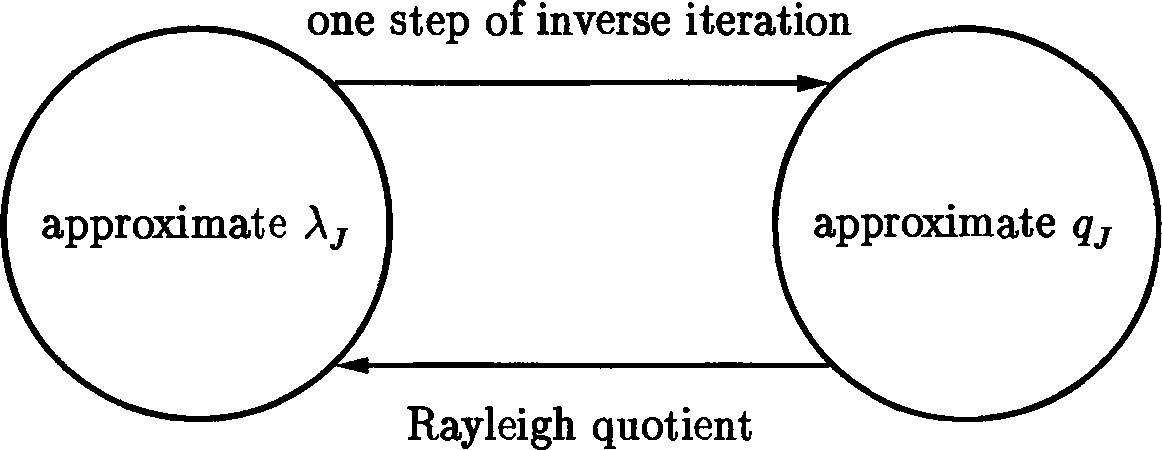
\includegraphics[width=0.83\linewidth]{../assets/figure-27-rayleigh-cycle.png}
    \caption{Rayleigh 商迭代的思想：一次逆迭代把特征值估计变成特征向量估计，
    Rayleigh 商再把特征向量估计变回特征值估计。原书特别说明该图是简化示意；
    从近似 $\lambda_J$ 得到近似 $q_J$ 还需要一个初始的 $q_J$ 近似。}
\end{figure}

这个想法是：不断改进特征值估计，从而在每一步提高逆迭代的收敛速率。所得
算法称为 Rayleigh 商迭代。

\paragraph{算法 27.3（Rayleigh 商迭代）}
\begin{verbatim}
v^(0) = some vector with ||v^(0)|| = 1
lambda^(0) = (v^(0))^T A v^(0) = corresponding Rayleigh quotient
for k = 1, 2, ...
      Solve (A - lambda^(k-1) I) w = v^(k-1) for w
          apply (A - lambda^(k-1) I)^(-1)
      v^(k) = w / ||w||                           normalize
      lambda^(k) = (v^(k))^T A v^(k)              Rayleigh quotient
\end{verbatim}

这个算法的收敛速度极其惊人：每次迭代都会把准确数字的数量大致提高到原来的
三倍。

\paragraph{定理 27.3.}
Rayleigh 商迭代对除一个测度为零的初始向量集合之外的所有
$v^{(0)}$，都收敛到一个特征值/特征向量对。若它收敛，并且 $\lambda_J$ 是
$A$ 的特征值、$v^{(0)}$ 足够接近特征向量 $q_J$，则最终具有三次收敛性：

\begin{equation}
\|v^{(k+1)}-(\pm q_J)\|
 =O\left(\|v^{(k)}-(\pm q_J)\|^3\right),
\tag{27.6}
\end{equation}

以及

\begin{equation}
|\lambda^{(k+1)}-\lambda_J|
 =O\left(|\lambda^{(k)}-\lambda_J|^3\right),
\tag{27.7}
\end{equation}

当 $k\to\infty$ 时成立。式 (27.6) 两侧的 $\pm$ 不一定相同。

这里不证明“几乎所有初始向量都会收敛”的断言，只证明一旦收敛就最终三次
收敛。为简单起见，假设 $\lambda_J$ 是单特征值。由 (27.3)，如果
$\|v^{(k)}-q_J\|<\epsilon$ 且 $\epsilon$ 足够小，那么 Rayleigh 商给出
一个满足

\[
|\lambda^{(k)}-\lambda_J|=O(\epsilon^2)
\]

的特征值估计。随后从 $v^{(k)}$ 和 $\lambda^{(k)}$ 出发做一步逆迭代，
得到新的 $v^{(k+1)}$，于是

\[
\|v^{(k+1)}-q_J\|
 =O\bigl(|\lambda^{(k)}-\lambda_J|\,\|v^{(k)}-q_J\|\bigr)
 =O(\epsilon^3).
\]

$O$ 符号中的常数在 $\lambda_J$ 和 $q_J$ 的充分小邻域内是一致的。因此，
误差会按照下面的模式推进：

\[
\begin{array}{c@{\qquad}c}
\|v^{(k)}-(\pm q_J)\| & |\lambda^{(k)}-\lambda_J|\\
\epsilon & O(\epsilon^2)\\
\downarrow\searrow & \\[-2pt]
O(\epsilon^3) & O(\epsilon^6)\\
\downarrow\searrow & \\[-2pt]
O(\epsilon^9) & O(\epsilon^{18})\\
\vdots & \vdots
\end{array}
\]

式 (27.6)–(27.7) 就由上述一致性得到。

\paragraph{例 27.1（三次收敛的数值例子）}
考虑对称矩阵

\[
A=\begin{bmatrix}
2&1&1\\
1&3&1\\
1&1&4
\end{bmatrix},
\qquad
v^{(0)}=\frac{(1,1,1)^T}{\sqrt3}.
\]

对 $A$ 使用 Rayleigh 商迭代，前三次迭代得到

\[
\lambda^{(0)}=5,\qquad
\lambda^{(1)}=5.2131\ldots,\qquad
\lambda^{(2)}=5.214319743184\ldots.
\]

与 $v^{(0)}$ 最接近的特征向量对应的真实特征值为
$\lambda=5.214319743377$。只经过三次迭代，Rayleigh 商迭代就得到了约十位
有效数字；如果机器精度足够高，再进行三次迭代，准确数字大约会增加到 270 位。

\section*{运算量}

最后估计上述三种迭代每一步所需的工作量。

先设 $A\in\mathbb{R}^{m\times m}$ 是满矩阵。幂迭代的每一步包含一次矩阵--
向量乘法，需要 $O(m^2)$ 次浮点运算。逆迭代的每一步需要解一个线性系统，
表面上似乎需要 $O(m^3)$ 次运算；但如果事先用 LU 分解、QR 分解或其他方法
处理矩阵，这个工作量可以降到 $O(m^2)$。Rayleigh 商迭代中每一步待求逆的
矩阵都会改变，因此要把每步的工作量降到 $O(m^3)$ 以下并不直接。

如果 $A$ 是三对角矩阵，情况会大大改善：现在三种迭代每一步都只需要
$O(m)$ 次浮点运算。顺便指出，对于涉及非对称矩阵的相应迭代，我们要处理的
是 Hessenberg 结构而不是三对角结构，工作量会增加到 $O(m^2)$。

\section*{习题}

\paragraph{27.1.}
设 $A\in\mathbb{C}^{m\times m}$，不一定是 Hermitian 矩阵。证明：复数
$z\in\mathbb{C}$ 是 $A$ 的某个 Rayleigh 商，当且仅当它是某个酉矩阵 $Q$
变换后的矩阵 $Q^*AQ$ 的一个对角条目。也就是说，只要把坐标系正交地变换
到合适的位置，Rayleigh 商正好就是矩阵的对角条目。

\paragraph{27.2.}
仍设 $A\in\mathbb{C}^{m\times m}$ 任意。所有非零向量 $x\in\mathbb{C}^m$
对应的 Rayleigh 商组成的集合称为 $A$ 的值域或数值域，记为 $W(A)$，
它是复平面的一个子集。

\begin{enumerate}[label=(\alph*)]
  \item 证明 $W(A)$ 包含 $A$ 的特征值的凸包。
  \item 证明如果 $A$ 是正规矩阵，那么 $W(A)$ 等于 $A$ 的特征值的凸包。
\end{enumerate}

\paragraph{27.3.}
证明：对于非 Hermitian 矩阵 $A\in\mathbb{C}^{m\times m}$，Rayleigh 商
$r(x)$ 给出的特征值估计通常只有线性精度，而不是二次精度。说明这会暗示
Rayleigh 商迭代具有怎样的收敛速率。

\paragraph{27.4.}
每个实对称方阵都可以正交对角化，而且本讲的推导在正交坐标变换下保持不变。
因此，原本可以一开始就假设 $A$ 是一个对角矩阵，并且对角条目按绝对值递减
排列。在这个假设下，描述式 (27.4)、(27.5) 和算法 27.3 的具体形式。

\paragraph{27.5.}
如正文所述，逆迭代依赖于求解一个可能极度病态的线性系统，其条件数可能达到
$\epsmach^{-1}$ 的量级。我们知道，一般不可能准确求解病态系统；这难道不是
算法的致命缺陷吗？

证明答案是否定的：病态性并不是逆迭代的问题。设 $A$ 是实对称矩阵，并且有
一个特征值的绝对值远小于其余特征值（不妨取 $\mu=0$）。设 $v$ 在 $A$ 的
所有特征向量 $q_1,\ldots,q_m$ 的方向上都有分量，并且 $Aw=v$ 采用后向稳定
方法求解，得到计算向量 $\widetilde w$。利用第 95 页的计算，证明虽然
$\widetilde w$ 可能与 $w$ 相差很远，但
$\widetilde w/\|\widetilde w\|$ 不会与 $w/\|w\|$ 相差很远。

\paragraph{27.6.}
如果 $A$ 的两个特征值相等，图 27.1 会发生什么变化？

\end{document}
